% !TEX encoding = UTF-8
% !TEX program = pdflatex
% !TEX root = relazione.tex
% !TeX spellcheck = it_IT

% ESEMPI
\section{Esempi}\label{sec:esempi}
Parlando di riconoscimenti visivo, è naturale inserire anche alcuni esempi su immagini di prova per mettere a confronto
le diverse piattaforme nei casi specifici.
Sono state identificate quattro funzionalità presenti in tutti i servizi (come si può vedere dalla tabella~\ref{tab:riass-funzionalita} in appendice):
riconoscimento di oggetti specifici, il riconscimento di scene e il riconscimento di volti.

Per consentire la maggior imparzialità, le immagini sono state selezionate casualmente da alcuni motori di ricerca.
%
\subsection{Riconoscimento di un oggetto specifico}\label{subsec:riconscimento-oggetto-specifico}
L'immagine presa come riferimento è la figura~\ref{fig:scontrino} che raffigura uno scontrino fiscale.
\begin{figure}[!h]
\begin{center}
	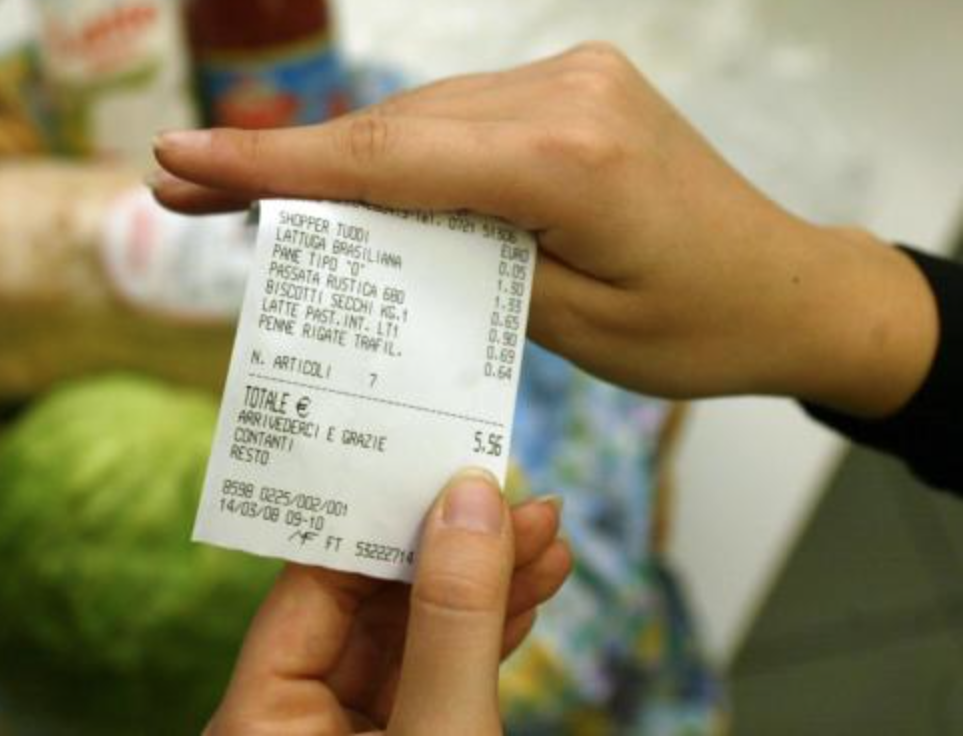
\includegraphics[scale=.5]{scontrino.png}
{\scriptsize \caption{Immagine usata come riferimento.}
\label{fig:scontrino}}
\end{center}
\end{figure}
%
\paragraph{Microsoft} Utilizzando le Computer Vision API con i metodi di tagging, classificazione e generazione di descrizioni,
il risultato ottenuto è\footnote{Alcuni campi, non direttamente rilevanti, sono stati omessi per faciltare la lettura.}:
%
\begin{lstlisting}[style=myJSON, caption=Risultato dell'interrogazione con le Computer Vision API., label=lst:risultati-microsoft-scontrino]
{
   'categories':[{
         'name':'text_menu',
         'score':0.85546875
    }],
   'description':{
      'captions':[{
            'confidence':0.6941834877564524,
            'text':'a close up of a receipt'
         }],
      'tags':['text', 'receipt']
   },
   'tags':[
      {'confidence':0.9944400787353516,
         'name':'text'},
      {'confidence':0.9528059959411621,
         'name':'receipt'}]
}
\end{lstlisting}
%
Come si può vedere, l'immagine viene classificata come \textsf{menu} nella categoria \textsf{text} (della macro-categoria \textsf{object});
considerando che in tutto ci sono meno di 90 categorie (per la tassonomia vedere la sezione~\ref{subsec:computer-vision-api}), il risultato è piuttosto soddisfacente.
Descrive l'immagine come: ``Un primo piano di uno scontrino'', quindi è decisamente esatta.
Infine, fornisce l'etichetta \textsf{testo} con un livello di affidabilità del $99,44\%$ e \textsf{scontrino} con il $95,28\%$.
Riassumendo, il sistema riconosce perfettamente l'oggetto nel suo complesso, anche se non ci fornisce particolari dettagli.
%%
\subsection{Riconoscimento di volti}\label{subsec:riconscimento-volti}
% In questo caso, l'immagine~\ref{fig:stallone} raffigura due personaggi famosi. Questo forse potrebbe facilitare il riconoscimento
% considerando che una caratteristica offerta (in tutte le piattaforme) è il riconoscimento di persone famose.
%
\begin{figure}[!h]
\begin{center}
	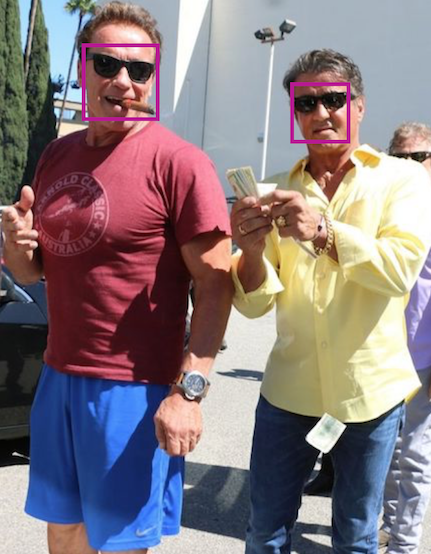
\includegraphics[width=150px,height=193px]{Sylvester-Stallone-making-it-rain-on-pal-Arnold-Schwarzenegger_microsoft.png}
	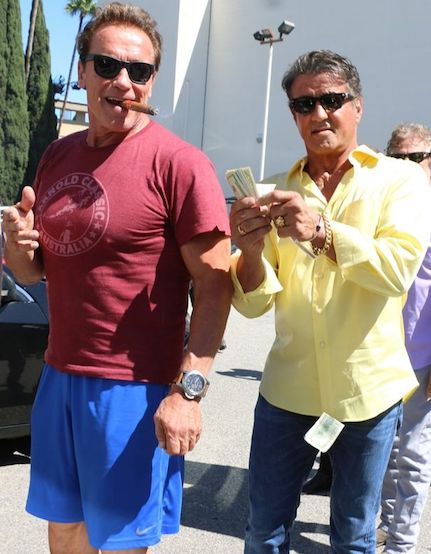
\includegraphics[width=150px,height=193px]{Sylvester-Stallone-making-it-rain-on-pal-Arnold-Schwarzenegger.jpg}
	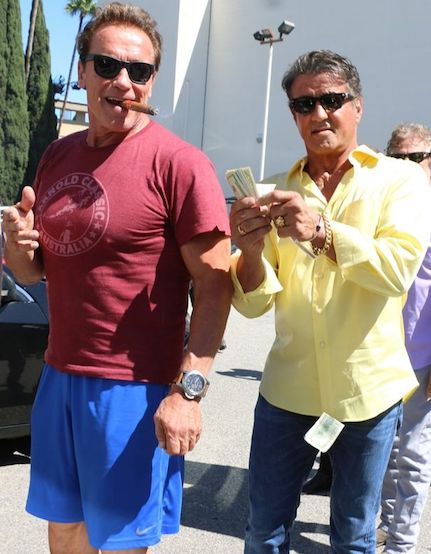
\includegraphics[width=150px,height=193px]{Sylvester-Stallone-making-it-rain-on-pal-Arnold-Schwarzenegger.jpg}
	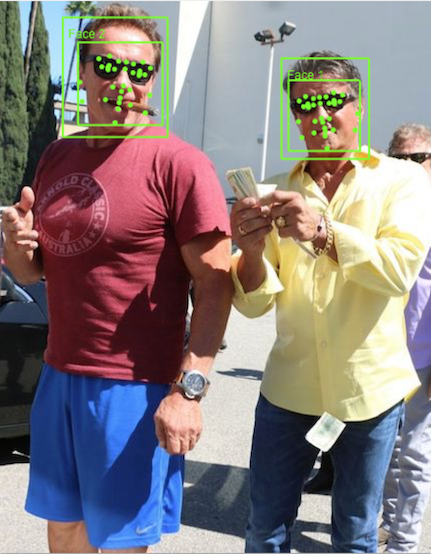
\includegraphics[width=150px,height=193px]{Sylvester-Stallone-making-it-rain-on-pal-Arnold-Schwarzenegger_google.png}
{\scriptsize \caption{Riconscimento dei volti utilizzando le quattro piattaforme.}
\label{fig:riconscimento-volti}}
\end{center}
\end{figure}
